\section{Types of network representations}
\label{sec:ch4:net-rep}

Now that you know how to represent networks with matrices and have some ideas of properties of networks, let's take a step back and take a look at what network representation is in general, and the different ways you might think about representing networks to understand different aspects of the network.

We already know that the topological structure of networks is just a collection of nodes, with pairs of nodes potentially linked together by edges. Mathematically, this means that a network is defined by two objects: the set of nodes, and the set of edges, with each edge just being defined as a pair of nodes for undirected networks. Networks can have additional structure: you might have extra information about each node (``features'' or ``covariates''), which we'll talk about when we cover Joint Representation Learning in Section \ref{sec:ch6:joint}. Edges might also have weights, which are usually measure the connection strength in some way. We learned in the previous section that network topology can be represented with matrices in a number of ways -- with adjacency matrices, Laplacians, or (less commonly) with incidence matrices. 

One major challenge in working with networks is that a lot of standard mathematical operations and metrics remain undefined. What does it mean to add a network to another network, for instance? How would network multiplication work? How do you divide a network by the number 6? Without these kinds of basic operations and metrics, you are left in the dark when you try to find analogies to non-network data analysis.

Another major challenge has to do with the nature of network data. As it turns out, for any given number of nodes, there are a finite number of possible networks. When you have a finite number of possible outcomes, one of the most natural approaches is to attempt to use the data to try to describe each possible outcome individually. For instance, if you are flipping a coin, you might try to use the data (coin flips that you see) to determine with which probability the coin lands on heads or tails, since heads and tails are the two possible outcomes of the coin flip.

Unfortunately, we cannot possibly do this for network data. When a simple network has $n$ nodes, the number of possible networks that you could observe is $2^{\binom n 2}$ (we will derive this result later in Section \ref{sec:ch5:er}). We plot what this looks like in Figure \ref{fig:ch4:nnets}. When you allow for only 50 nodes, there are already more than $10^{350}$ possible networks. Just for reference, it is estimated that there are $10^{80}$ atoms in the known universe. If you created $10^{80}$ new universes, each with $10^{80}$ atoms, the total number of atoms across all universes would still be nowhere near this amount. 

In this section, we will explore the ways in which we conceptualize network representations to overcome this limitation. This section will prepare you to conceptualize the many particular strategies that you will learn later in Chapters \ref{sec:ch5} and \ref{sec:ch6}.

\begin{figure}[h]
    \centering
    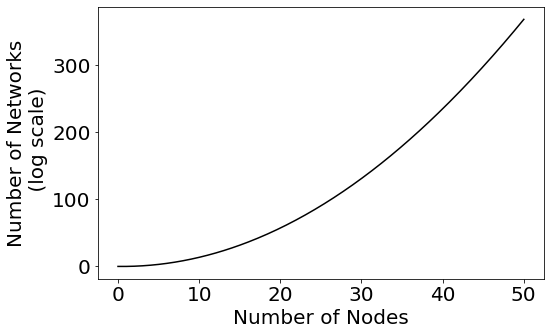
\includegraphics[width=0.7\linewidth]{representations/ch4/Images/nnets.png}
    \caption[Number of networks for $n$ nodes]{The number of possible distinct networks that you could have for a given number of nodes.}
    \label{fig:ch4:nnets}
\end{figure}

\subsection{Bag of Features}

The first approach is called the bag of features. The idea is that you take networks and you compute statistics from them, either for each node or for the entire network. These statistics could be simple things like the edge count or average path length between two nodes like you learned about in the last section, or more complicated metrics like the modularity \cite{Newman2006Jun}, which measures how well a network can be separated into communities. Unfortunately, network statistics like these tend to be correlated; the value of one network statistic will almost always influence the other. This means that it can be difficult to interpret analysis that works by comparing network statistics. It's also hard to figure out which statistics to compute, since there are an infinite number of them.

\subsubsection{You Lose A Lot of Information with the Bag of Features Approach}

Let's take a look at a collection of networks in Figure \ref{fig:ch4:anascombe}:

\begin{figure}[h]
    \centering
    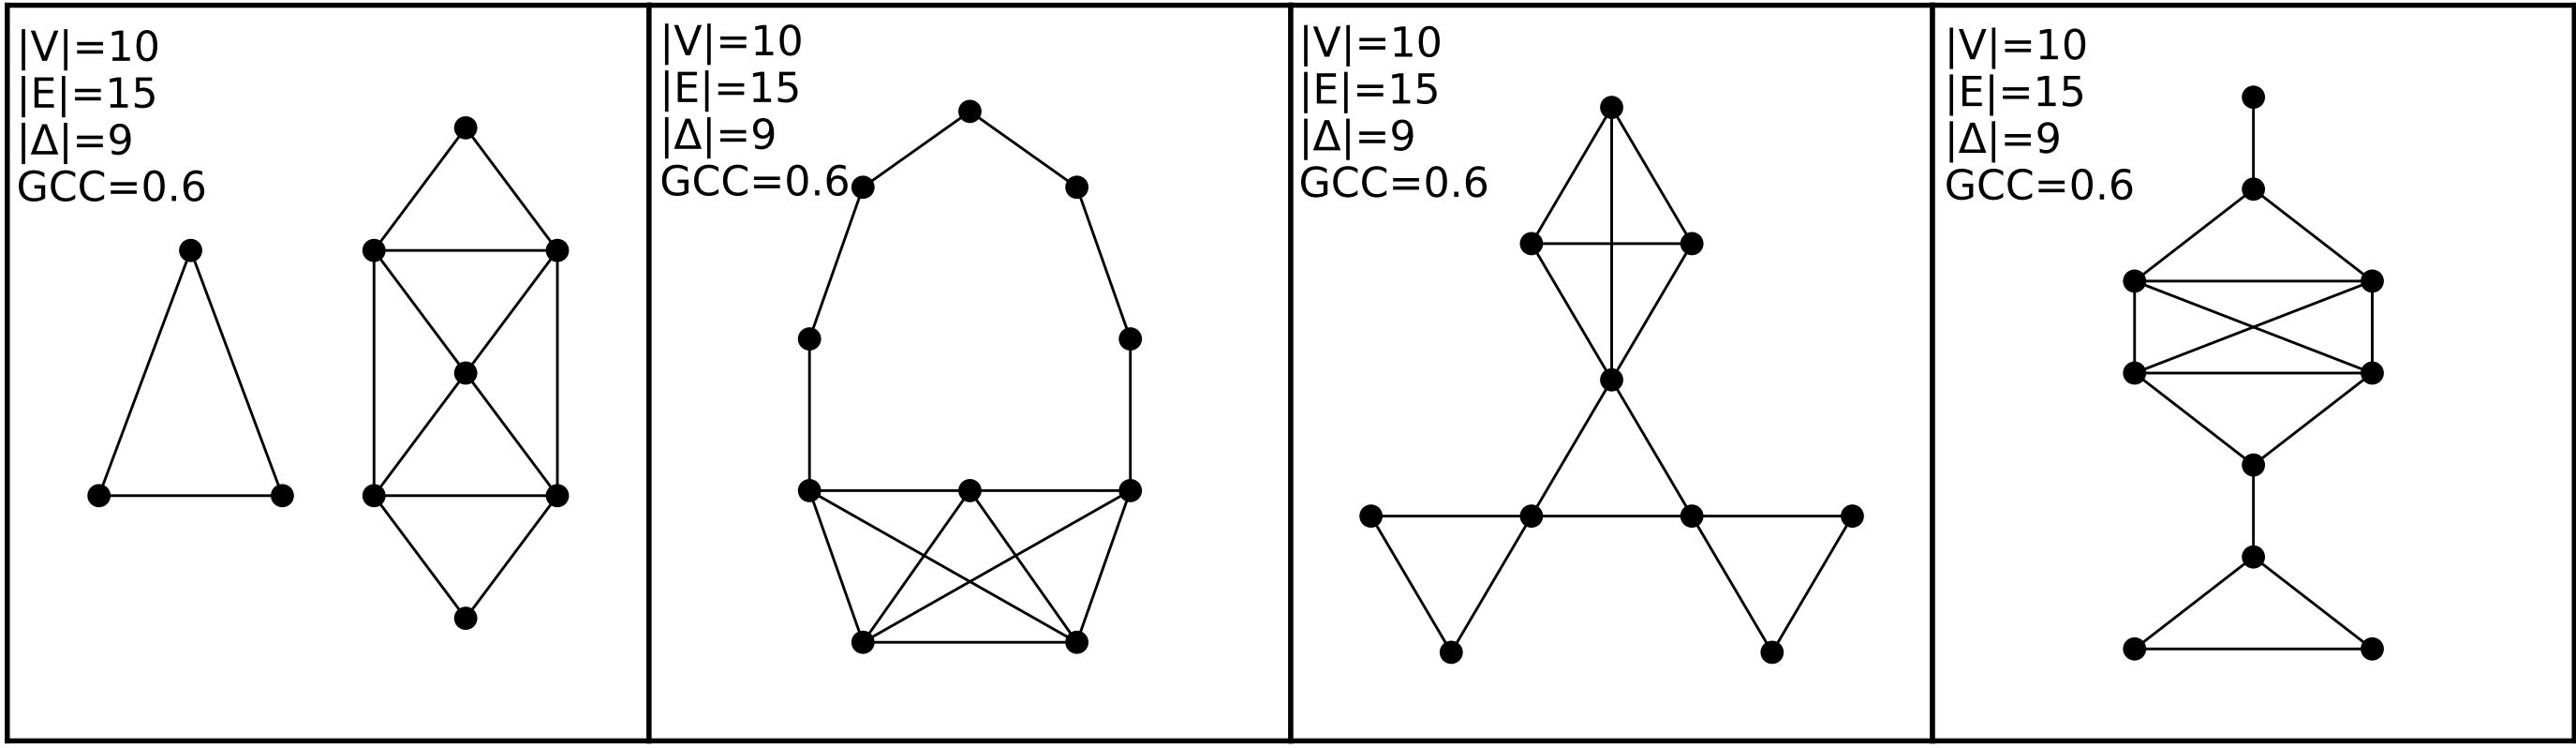
\includegraphics[width=\linewidth]{representations/ch4/Images/anascombe.jpeg}
    \caption[Very different networks can have the same summary statistics]{Four networks, all of which have the exact same network statistics for the four statistics we show here. They each have ten nodes and 15 edges. They also all contain the same number of closed triangles, and the same global clustering coefficient from Section \ref{sec:ch4:prop-net:clustering}.}
    \label{fig:ch4:anascombe}
\end{figure}

These networks all have the same basic network statistics. Each of these networks, however, are completely different from each other. The first network, for instance, has two connected components, while the others are all connected. The second network has a community of nodes that are only connected along a path, and a different community which are tightly connected, and so on. Modeling these networks through computing these features from them would lose a great deal of useful information about the topology of the network.


\paragraph{Network Features Tend to be Correlated}
\label{sec:ch4:net-rep:featurelims}

As we mentioned in the last paragraph, if you consider all possible networks, knowing the value of any of the network features gives you information about what the value of other network features might be.

Let's play around with this. We'll make $100$ random networks, each with $50$ nodes, and then we'll compute some common network statistics that people use in practice. Then, we'll look at how correlated these features are. For now, just think of a random network as being a network with each node being connected to each other node with some probability. Each network will have a different connection probability. These networks also might have communities --- groups of nodes which have similar connection probabilities of being connected with other groups of nodes. 

Conceptually, you could think about a particular type of community structure using the bridge example that we covered previously when we talked about the Boston and New York boroughs in the LCC example in Section \ref{sec:ch4:prop-net:lcc}. It is probably more likely that two boroughs that are in the same state have a bridge between them than two boroughs in totally different states, right? When you generate data later on in this book, we'll get into different types of network models you can use. You don't need to have too good of an idea of what the below simulation code is doing just yet --- we will go into more depth in Chapter \ref{sec:ch5}.

\begin{lstlisting}[style=python]
from graspologic.simulations import sbm
import numpy as np
from numpy.random import uniform

n_nodes = 50
n_networks = 100
np.random.seed(1234)
# within-community probability
p = uniform(size=100, low=.5).round(2)
# between-community probability
q = uniform(size=100, high=.5).round(2)

networks = []
for i in range(n_networks):
    np.random.seed(1234)
    P = np.array([[p[i], q[i]],
                  [q[i], p[i]]])
    network = sbm(n=[n_nodes//2, n_nodes//2], p=P)
    networks.append(network)
\end{lstlisting}
Now, for each of these networks, we'll calculate a set of network features, using some of the various properties you learned about in the previous Section \ref{sec:ch4:prop-net}.

The only new statistic that we will look at is known as the network \textit{modularity}. You don't need to know too much about this statistic right now, other than the fact that it quantifies how much ``stronger'' the within-community effect is than the between-community effect (basically, that idea we described that New York boroughs would be more likely to have a bridge to other New York boroughs, than with either of the two cities in Massachusetts). The other statistics that we will compute will be the network density, the clustering coefficient, and the path length, all of which we discussed in Section \ref{sec:ch4:prop-net}.

The code below defines functions to calculate each of these network features, and then calculates them for each of the networks you created above.

We'll also define a preprocessing decorator, which just converts the network from a numpy array into the format networkx uses.


\begin{lstlisting}[style=python]
import functools
import networkx as nx

def preprocess(f):
    @functools.wraps(f)
    def wrapper(network):
        network = nx.from_numpy_matrix(network)
        return f(network)
    return wrapper

@preprocess
def modularity(network):
    communities = nx.algorithms.community.greedy_modularity_communities(network)
    Q = nx.algorithms.community.quality.modularity(network, communities)
    return Q

@preprocess
def network_density(network):
    return nx.density(network)

@preprocess
def clustering_coefficient(network):
    return nx.transitivity(network)

@preprocess
def path_length(network):
    if nx.number_connected_components(network) != 1:
        # You want to make sure this still works if your network isn't fully connected!
        network = max((network.subgraph(c) for c in nx.connected_components(network)), 
                      key=len)
    return nx.average_shortest_path_length(network)
\end{lstlisting}

Now, we'll calculate all of these features for each network, and finally we'll create a heatmap of their correlation.

\begin{lstlisting}[style=python]
import pandas as pd

network_features = []
for i, network in enumerate(networks):
    modularity_ = modularity(network)
    network_density_ = network_density(network)
    clustering_coefficient_ = clustering_coefficient(network)
    path_length_ = path_length(network)
    features = {"Modularity": modularity_, "Network Density": network_density_, 
                "Clustering Coefficient": clustering_coefficient_, "Average Path Length": path_length_}
    network_features.append(features)
    
df = pd.DataFrame(network_features)
feature_correlation = df.corr()
\end{lstlisting}
We show the results of this plot in Figure \ref{fig:ch4:anascombe}. Numbers close to 1 mean that when the first feature is large, the second tends to be large, numbers close to 0 mean that the features are not very correlated, and numbers close to -1 mean that when the first feature is large, the second feature tends to be small. 

\begin{figure}[h]
    \centering
    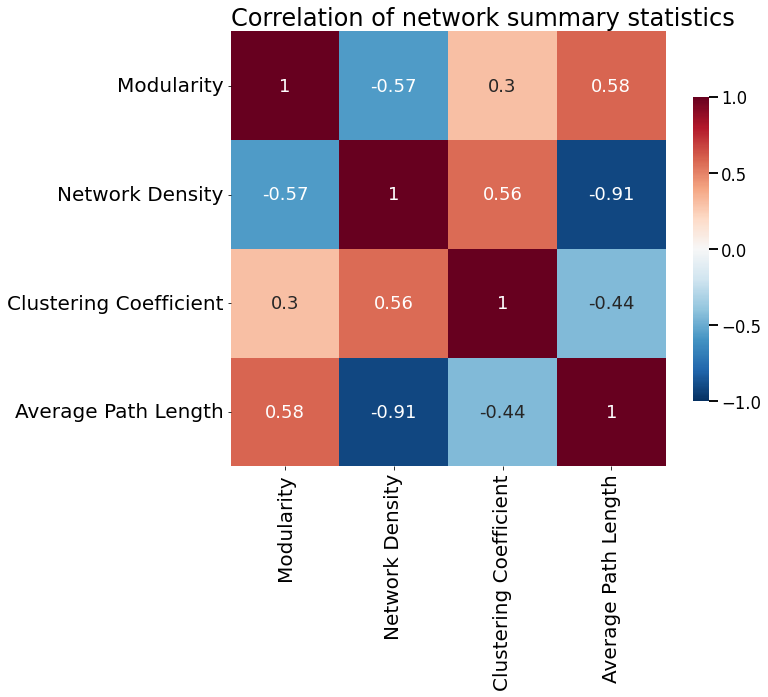
\includegraphics[width=0.8\linewidth]{representations/ch4/Images/corr.png}
    \caption[Correlation of netework features experiment]{The networks tend to exhibit correlation across various summary statistics. Note that none of the correlations are particularly close to $0$, and some (such as path length and density) are nearly perfectly correlated/anti-correlated.}
    \label{fig:ch4:corr}
\end{figure}

If you're familiar with correlation, that these numbers aren't particularly close to zero means that many of the features contain varying degrees of information about other features. Some of these features being big might say that another feature tends to also be high (positive correlation). Some of these features being big might say that another feature might tend to be the small (negative correlation). Some of these features don't tell you much about another particular feature (for instance, clustering and modularity only have a correlation with a magnitude around $0.3$), and some features are nearly perfectly informative about other features (network density and average path length are nearly perfectly negative-correlated with a value of $-.91$; that is, a high average path length implies a low network density, and vice versa). 

\paragraph{Why Network Feature Correlatedness Can Lead To Problems}

Let's take a step back to the implications of using the bag of features approach to analyze networks, now that you can see how correlated they usually are. Say you have a bunch of brain networks of mice, where the nodes are neurons and the edges are connections between neurons. You have a group of mice who were raised total darkness, and another group who were raised normally: let's call the ones who were raised in the darkness the batman mice. You're interested in how the visual parts of the brain are affected in the batman mice. You find the networks for only the visual parts of their brain, and then you calculate some network feature; maybe the density. It turns out that the network density is much lower for batman mice than it is for normal mice, so you conclude that raising mice in the darkness causes lower network density. Seems reasonable.

The problem is that network density is correlated with pretty much every other network feature you could have used. When you perform science, a primary focus of science tends to be establishing \textit{causality}. While we won't go much into causality here (there is an entire field dedicated to just this topic, called {causal inference}  for which there are many stellar reference texts), the jist is this. When you try to establish causality, you want to show a cause and effect type of relationship: the presence, or lack thereof, of some item $X$ {causes} an outcome $Y$ to happen. Whenever you do science, you want to find the root causes of {why} something is what it is: a mental illness is caused by a misfiring neuron, a misfolded protein is caused by the absence of a particular amino acid, a pair of friends having a major fight led to the students in a school being separated friendship wise into two distinct groups of people who support one student or the other. What you don't want to do is find something that just happens to be {correlated} with the thing that is impacted. 

For an example of this, we'll rotate back to our example from Section \ref{sec:ch1:howstudy:wontdiscuss}. If all smokers were older people and all non-smokers were younger people, just observing that the smokers tended to have higher rates of lung cancer would be insufficient to conclude whether smoking, or aging, cause lung cancer. Fortunately, statisticians found a way out: they took large groups of people with similar age ranges (and a number of other factors), and showed that the smokers had higher cancer rates (thus, ``untangling'' the correlatedness of age and smoking status). 

When you look at network features as things that potentially ``cause'' a particular effect, you can't really ``untangle'' the correlatedness of these network features, and it becomes extremely difficult, if not {impossible}  to actually establish which aspects of the network topology are actually causing or effected by the factor you are studying. 

For this reason, we think that network features are useful to {ascertain} whether something has an effect on the network, and provide information as to which directions you might want to look to establish causality. However, network features alone are insufficient, in our opinion, for defining causality. 

\subsection{Bag of Edges}
\label{sec:ch4:net-rep:bagofedges}

The second approach to studying networks is called the bag of edges. Here, you just take all of the edges in your network and treat them all as independent entities. You study each edge individually, ignoring any interactions between edges. This can work in some situations, but you still run into dependence: if two people within a friend group are friends, that can change the dynamic of the friend group and so change the chance that a different set of two people within the group are friends.

More specifically, in the bag of edges approach, you generally assume that every edge in your network will exist with some particular {probability} which can be different depending on the edge that you're looking at. For example, there might be a 60\% chance that the first and second nodes in your network are connected, but only a 20\% chance that the third and fourth nodes are. What often will happen here is that you have multiple networks describing the same (or similar) systems. For example, let's use the mouse example again from above. You have your batman mice (who were raised in the dark) and your normal mice. You'll have a network for each batman mouse and a network for each normal mouse, and you assume that, even though there's a bit of variation in what you actually see, the {probability} of an edge existing between the same two nodes is the same for all batman mice. Your goal would be to figure out which edges have a different {probability} of existing with the batman mice compared to the normal mice.

Let's make some example networks to explore this. We'll have two groups of networks, and all of the networks will have only three nodes for simplicity's sake. Each group will contain 20 networks, for a total of 40 networks. In the first group, every edge between every pair of nodes simply has a 50\% chance of existing. In the second group, the edge between nodes 0 and 1 will instead have a 90\% chance of existing, but every other edge will still just be 50\%. We'll generate ten networks from the first group, and ten networks from the second group.

\begin{lstlisting}[style=python]
from graspologic.simulations import sample_edges

P1 = np.array([[.5, .5, .5],
               [.5, .5, .5],
               [.5, .5, .5]])

P2 = np.array([[.5, .9, .5],
               [.9, .5, .5],
               [.5, .5, .5]])

# First group
n_networks = 20
networks = np.empty((2*n_networks, 3, 3))
for i in range(n_networks):
    networks[i,:,:] = sample_edges(P1)

# Second group
for i in range(n_networks, 2*n_networks):
    networks[i,:,:] = sample_edges(P2)

ys = np.array([1 for i in range(0, n_networks)] + [2 for i in range(0, n_networks)])
\end{lstlisting}

\subsubsection{Figuring out which edge is the signal edge}

By design, you know that the edge between nodes 0 and 1 has signal - the probability that it's there changes depending on whether your network is in the first or the second group. One common goal when using the bag of edges approach is finding signal edges: edges whose probability of existing changes depending on which type of network you're looking at. In your case, we're trying to figure out (without using your prior knowledge) that the edge between nodes 0 and 1 is a signal edge.

To find the outlier edge, you'll first get the set of all edges, along with their indices. Since all of your networks are undirected, you'll get the edges and their indices by finding all of the values in the the upper-triangular portion of the adjacency matrices.

\begin{lstlisting}[style=python]
edge_indices = np.triu_indices(3, k=1)
\end{lstlisting}

Now, you'll use a hypothesis test called the {Fisher's Exact Test} to find the outlier edge. You don't need to worry too much about what fisher's exact test is; here it is just something that will let us quantify whether an edge is different between the two groups, while makes limited assumptions about your data. We'll talk more about it in Section \ref{sec:ch9:ssn_incoherent}. 

In the code below, we:
\begin{enumerate}
    \item Loop through the edge indices,
    \item Get a list of all instances of that edge in the first group, and all instances of that edge in the second group, and
    \item Feed that list into the Fisher's exact test and obtain $p$-values (small $p$-value = more signal).
\end{enumerate}

\begin{lstlisting}[style=python]
from scipy.stats import fisher_exact

edge_pvals = []
for i, j in zip(*edge_indices):
    gr1_edge = networks[ys == 1,i,j].sum()  # number of group1 with edge i,j
    gr2_edge = networks[ys == 2,i,j].sum()  # number of group2 with edge i,j
    gr1_noedge = n_networks - gr1_edge  # number of group1 without edge i,j
    gr2_noedge = n_networks - gr2_edge  # number of group2 without edge i,j
    
    edge_tab = np.array([[gr1_edge, gr2_edge], [gr1_noedge, gr2_noedge]])  # arrange as in table
    
    edge_pvals.append(fisher_exact(edge_tab).pvalue)
\end{lstlisting}
You can see below that the $p$-value for the first edge, the one that connects nodes 0 and 1, is extremely small, whereas the $p$-values for the other two edges are relatively large.

\begin{lstlisting}[style=python]
np.array(edge_pvals).round(3)
\end{lstlisting}

\subsection{Bag of Nodes}
\label{sec:ch4:net-rep:bagofnodes}

Similarly to the bag of edges, you can treat all of the nodes as their own entity and do analysis on a bag of nodes. Much of this book will focus on the bag of nodes approach, because we'll often use edge count, covariate information, and other things when we work with bags of nodes. Although there's still correlation between nodes, it generally isn't as big of an issue. Most of the single-network methods you'll use in this book will take the bag of nodes approach. 

What we'll see repeatedly is that we take the nodes of a network and {embed} them so each node is associated with a point on a plot (this is called the {node latent space}). In a sense, this will ``tabularize'' our data, which as we learned in Section \ref{sec:ch1:challenges}, overcomes a major hurdle of network machine learning. Then, we can use other methods from mainstream machine learning to learn about our network. Deciding how to handle these ``bags of nodes'' will be a prime focus of Chapter \ref{sec:ch6}, and we will devote attention in Part \ref{p:app} to determining how we can use these bags of nodes.

We'll also often associate node representation with community investigation. The idea is that sometimes you have groups of nodes which behave similarly -- maybe they have a higher chance of being connected to each other, or maybe they're all connected to certain other groups of nodes. Regardless of how you define communities, a community investigation motif will pop up: you get your node representation, then you associate nearby nodes to the same community. We can then look at the properties of the node belonging to a particular community, or look at relationships between communities of nodes.

Since we'll use the bag of nodes approach heavily throughout this book, you'll be getting a much better sense for what you can do with it later. As a sneak preview right now, let's generate a few networks and embed their nodes to get a feel for what bag-of-nodes type analysis might look like. 

Don't worry about the specifics, but below you generate a simple network with two communities. Nodes in the same community have an 80\% chance of being connected, whereas nodes in separate communities have a 20\% chance of being connected. This is like saying that boroughs of New York \textit{or} boroughs near Boston have an 80\% of being connected by bridges, but boroughs of New York and boroughs near Boston have a 20\% chance of having a bridge between them. There are 20 nodes per community. Again, we'll cover the intuition of this particular generative model a lot more in Chapter \ref{sec:ch5}, so keep the big picture in focus for now.

\begin{lstlisting}[style=python]
from graspologic.simulations import sbm

# generate network
P = np.array([[.8, .2,],
              [.2, .8]])
network, labels = sbm(p=P, n=[20, 20], return_labels=True)
\end{lstlisting}

Now, you'll use graspologic to find the points in 2D space that each node is associated with. Again, don't worry about the specifics: this will be heavily explained later in the book. All you have to know right now is that we're {mapping} (transforming) the nodes of your network from network space, where each node is associated with a set of edges with other nodes, to the a tabular space, where each node is associated with an $x$-coordinate and a $y$-coordinate.

\begin{lstlisting}[style=python]
from graspologic.embed import AdjacencySpectralEmbed as ASE

ase = ASE(n_components=2)
embedding = ase.fit_transform(network)
\end{lstlisting}

Figure \ref{fig:ch4:bagonode} shows the result of this tabularization by community. Each of the dots in this plot is one of the nodes of your network. You can see that the nodes cluster into two groups: one group for the first community, and another group for the second community. Using this representation for the nodes of your network, you can open the door to later downstream machine learning tasks.

\begin{lstlisting}[style=python]
from graphbook_code import plot_latents, draw_cartesian, add_circle, text

ax = draw_cartesian(xrange=(-1, 1), yrange=(-1, 1))
plot = plot_latents(embedding, labels=labels, ax=ax)
plot.set_title("Bag of Nodes on a coordinate axis", y=1.1);

# plot circle
x_centroid, y_centroid = embedding[labels==0].mean(axis=0)
add_circle(x_centroid, y_centroid+.2, ax=ax)
ax.annotate("Nodes plotted \nas 2d points", xy=(x_centroid-.2, y_centroid+.2), xytext=(x_centroid-2, y_centroid), 
            arrowprops={"arrowstyle": "->"});
\end{lstlisting}
\begin{figure}[h]
    \centering
    \includegraphics[width=\linewidth]{representations/ch4/Images/bagonode.png}
    \caption{Nodes in the same community ending up being in similar areas of the $x$/$y$ coordinate axis above.}
    \label{fig:ch4:bagonode}
\end{figure}

\subsection{Bag of Networks}
\label{sec:ch4:net-rep:bagofnets}

The last approach is the bag of networks, which you'd use when you have more than one network that you're working with. Here, you'd study the networks as a whole and you'd want to test for differences across different networks or classify entire networks into one category or another. You might want to figure out the groups of networks look different, or whether you can learn information across all of the networks simultaneously. This is can be useful if you have many extremely large networks, with millions of nodes.

To showcase the bag of networks approach, let's create a few networks. We'll have one group of networks distributed the same way, and another group distributed differently. What you want to do is plot each network as a point in space, so that you can see the communities of networks directly.

Both sets of networks will have two communities of nodes, but the first set will have slightly stronger within-community connections than the second. Each network will have 200 nodes in it, 100 for each community.

\begin{lstlisting}[style=python]
def make_network(*probs, n=100, return_labels=False):
    pa, pb, pc, pd = probs
    P = np.array([[pa, pb], 
                  [pc, pd]])
    
    return sbm([n, n], P, return_labels=return_labels)

n = 100
p1, p2, p3 = .12, .06, .03

first_group = []
for _ in range(6):
    network = make_network(p1, p3, p3, p1)
    first_group.append(network)
    
second_group = []
for _ in range(12):
    network = make_network(p2, p3, p3, p2)
    second_group.append(network)
\end{lstlisting}

Again, don't worry too much yet about the process with which these networks were generated - that will all be explained in the next chapter. All you need to get out of this code is that you have six networks from the first group, and another twelve networks from the second. You can see these networks in heatmap form below. These networks are plotted in Figure \ref{fig:ch4:bagonets}(A). 

Now, you have to figure out some way of plotting each network as a point in space. Here's a rough overview for how you'll do it.

First, you'll take all of your networks and find a common space that you can orient all of the nodes into. The nodes for all of the networks will exist in the same space, meaning their locations can be compared with each other. We'll have a bunch of matrices, one for each network. Since each network has 200 nodes, and we're embedding into 2-dimensional space, we'll have six 200 by 200 matrices for the first group of networks, and another twelve 200 by 200 matrices for the second group. This process is called finding a {network} latent space with a homogeneous {node latent space}  and will be extremely valuable for embedding collections of networks later on. Again, this takes our collection of networks and \textit{tabularizes} them for us, taking each $200 \times 200$ adjacency matrix and turning it into a $200 \times 2$ matrix, effectively ``bagging the nodes'' like we did in the preceding section.

Next, once we have a bag of nodes for each network, we can use standard machine learning techniques with them. Here, we'll use classical multi-dimensional scaling (MDS), a popular dimensionality reduction technique. We'll do this by constructing a dissimilarity matrix which captures how dissimilar each ``bag of nodes'' is between every pair of networks, and then embed this dissimilarity matrix. This second embedding, in effect, tabularizes each network individually and gives us a bag of networks representation.

Again, don't worry if you don't understand the details: embedding and how it works will be explained in future chapters.

\begin{lstlisting}[style=python]
from graspologic.embed import OmnibusEmbed as OMNI
from graspologic.embed import ClassicalMDS

# Find a node latent space for the nodes of all of your networks
omni = OMNI(n_components=2)
omni_embedding = omni.fit_transform(first_group + second_group)

# embed each network representation into a 2-dimensional space
cmds = ClassicalMDS(2)
cmds_embedding = cmds.fit_transform(omni_embedding)

# Find and normalize the dissimilarity matrix
distance_matrix = cmds.dissimilarity_matrix_ / np.max(cmds.dissimilarity_matrix_)
\end{lstlisting}

You can see the dissimilarity matrix in Figure \ref{fig:ch4:bagonets}(B). As you can see, there look to be two groups of networks that tend to be quite similar amongst themselves, and quite different between the groups. The diagonals of the matrix are all 0, because the dissimilarity between a network and itself is 0.

Embedding this {new} matrix will give us a point in space for each network. Once you find the embedding for this dissimilarity matrix via MDS as above, you can plot each of the networks in space. Since there are six networks of the first type and twelve of the second type, one of the clusters has six dots, and the other has twelve dots. Let's take a look at this plot:
\begin{lstlisting}[style=python]
ax = draw_cartesian(xrange=(-1, 1), yrange=(-1, 1))
labels = np.repeat([0, 1], [len(first_group), len(second_group)])
plot_latents(cmds_embedding, ax=ax, labels=labels, title="Networks plotted as 2d points")
\end{lstlisting}

\begin{figure}
    \centering
    \includegraphics[width=\linewidth]{representations/ch4/Images/bagonets.png}
    \caption[Bags of networks]{\textbf{(A)} the networks from each of the two groups. \textbf{(B)} The dissimilarity matrix between pairs of networks. \textbf{(C)} Each point represents a single network point in space. We can easily see the two clusters, which represent the two types of networks you created.}
    \label{fig:ch4:bagonets}
\end{figure}

\newpage